% Created 2020-09-21 lun 18:01
% Intended LaTeX compiler: pdflatex
\documentclass[presentation,aspectratio=169, usenames, dvipsnames]{beamer}
\usepackage[utf8]{inputenc}
\usepackage[T1]{fontenc}
\usepackage{graphicx}
\usepackage{grffile}
\usepackage{longtable}
\usepackage{wrapfig}
\usepackage{rotating}
\usepackage[normalem]{ulem}
\usepackage{amsmath}
\usepackage{textcomp}
\usepackage{amssymb}
\usepackage{capt-of}
\usepackage{hyperref}
\usepackage{khpreamble}
\usepackage{amssymb}
\usepgfplotslibrary{groupplots}
\usepackage{pgfplotstable}
\newcommand*{\shift}{\operatorname{q}}
\definecolor{ppc}{rgb}{0.1,0.1,0.6}
\definecolor{iic}{rgb}{0.6,0.1,0.1}
\definecolor{ddc}{rgb}{0.1,0.6,0.1}
\usetheme{default}
\author{Kjartan Halvorsen}
\date{2020-09-21}
\title{Process Automation Laboratory - Anti windup}
\hypersetup{
 pdfauthor={Kjartan Halvorsen},
 pdftitle={Process Automation Laboratory - Anti windup},
 pdfkeywords={},
 pdfsubject={},
 pdfcreator={Emacs 26.3 (Org mode 9.3.6)}, 
 pdflang={English}}
\begin{document}

\maketitle

\section{Context}
\label{sec:orgd19de8a}
\begin{frame}[label={sec:org69a135a}]{Two -tank model}
\begin{center}
\includegraphics[width=\linewidth]{../../figures/two-tanks-shutoff-valve}
\end{center}
\end{frame}

\section{Repetition PID}
\label{sec:org795dfcf}
\begin{frame}[label={sec:org9f8e291}]{Feedback control}
   \begin{center}
   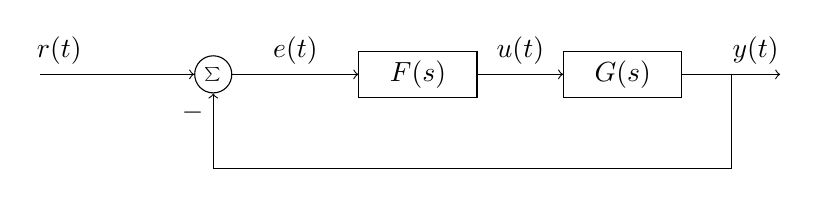
\begin{tikzpicture}[node distance=22mm, block/.style={rectangle, draw, minimum width=15mm}, sumnode/.style={circle, draw, inner sep=2pt}]
  { 
  \node[coordinate] (input) {};
  \node[sumnode, right of=input] (sum) {\tiny $\sum$};
  \node[block, right of=sum, node distance=2.6cm] (reg) {$F(s)$};
  \node[block, right of=reg, node distance=2.6cm] (plant) {$G(s)$};
  \node[coordinate, right of=plant, node distance=2cm] (output) {};
  \node[coordinate, below of=plant, node distance=12mm] (feedback) {};
 
  \draw[->] (plant) -- node[coordinate, inner sep=0pt] (meas) {} node[near end, above] {$y(t)$} (output);
  \draw[->] (meas) |- (feedback) -| node[very near end, left] {$-$} (sum);
  \draw[->] (input) -- node[very near start, above] {$r(t)$} (sum);
  \draw[->] (sum) -- node[above] {$e(t)$} (reg);
  \draw[->] (reg) -- node[above] {$u(t)$}(plant);
}
\end{tikzpicture}
\end{center}
\end{frame}



\begin{frame}[label={sec:org99d6d2f}]{The PID - practical form}
\definecolor{ppc}{rgb}{0.1,0.1,0.6}
\definecolor{iic}{rgb}{0.6,0.1,0.1}
\definecolor{ddc}{rgb}{0.1,0.5,0.1}

\begin{center}
  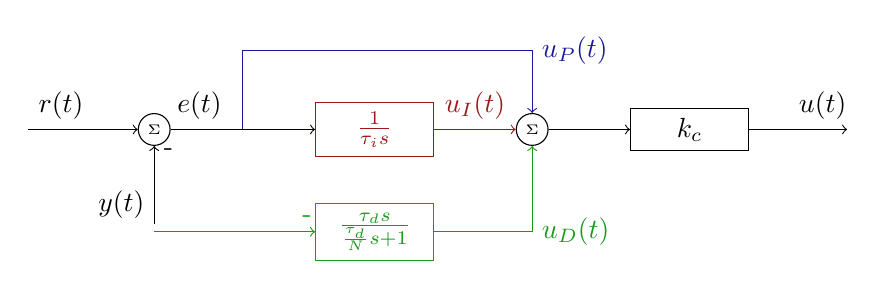
\begin{tikzpicture}[node distance=22mm, block/.style={rectangle, draw, minimum width=15mm}, sumnode/.style={circle, draw, inner sep=2pt}]

    \node[coordinate] (input) {};
    \node[sumnode, right of=input, node distance=16mm] (sum) {\tiny $\Sigma$};
    \node[color=iic,block, right of=sum, node distance=28mm] (ii)  {$\frac{1}{\tau_is}$};
    \node[color=ppc, coordinate, above of=ii, node distance=10mm] (pp)  {};
    \node[color=ddc,block, below of=ii, node distance=13mm] (dd)  {$\frac{\tau_ds}{\frac{\tau_d}{N}s + 1}$};
    \node[sumnode, right of=ii, node distance=20mm] (sum2) {\tiny $\Sigma$};
    \node[block, right of=sum2, node distance=20mm] (gain)  {$k_c$};
    \node[coordinate, below of=sum, node distance=12mm] (feedback) {};
    \node[coordinate, right of=gain, node distance=20mm] (output) {};

    \draw[->] (input) -- node[above, pos=0.3] {$r(t)$} (sum);
    \draw[->] (sum) -- node[above, pos=0.2] {$e(t)$} node[coordinate] (mm) {}  (ii);
    \draw[->] (gain) -- node[above, near end] {$u(t)$} (output);
    \draw[->] (feedback) -- node[left, near start] {$y(t)$} node[right, pos=0.95] {-} (sum);
    \draw[->, color=ppc] (mm) |- (pp) -| node[right,] {$u_P(t)$} (sum2);
    \draw[->, color=ddc] (feedback |- dd) -- node[above, pos=0.95] {-} (dd);
    \draw[->, color=ddc] (dd) -| node[right,] {$u_D(t)$} (sum2)  ;
    \draw[->, color=iic] (ii)  -- node[above,] {$u_I(t)$} (sum2);
    \draw[->] (sum2) -- node[above, near end] {} (gain);

  \end{tikzpicture}
\end{center}

The parameter \(N\) is chosen to limit the influence of noisy measurements. Typically,
\[  3 < N < 20 \]
\end{frame}

\begin{frame}[label={sec:org879c25a}]{The PID - practical aspects}
{\footnotesize Åström \& Hägglund (1988) \emph{PID controllers: Theory, design and tuning, 2nd ed} Instrument Society of America.}

\begin{block}{Approximating nonlinear systems with linear models}
\begin{itemize}
\item Model is accurate only in neighborhood of operating point for which system is approximated.
\item Solution: Divide operating range into many regions, with separate PID parameters for each region
\end{itemize}
\end{block}

\begin{block}{Approximating high-order systems with low-order models}
\begin{itemize}
\item Only accurate for low frequencies
\item Beware of behavior for high-frequency input to the closed-loop system
\end{itemize}
\end{block}
\end{frame}

\begin{frame}[label={sec:org2090f62}]{The PID - practical aspects, contd}
\begin{block}{When do PID controllers work well?}
\begin{itemize}
\item The plant dynamics can be well approximated with low-order model
\item Demands on performance not too high
\end{itemize}
\end{block}
\begin{block}{More sophisticated control needed when}
\begin{itemize}
\item Higher order dynamics
\item Oscillatory modes
\item Long deadtime
\end{itemize}
\end{block}
\end{frame}

\begin{frame}[label={sec:org2acf1f0}]{The PID - practical aspects, contd}
\begin{block}{Choice of controller}
\begin{enumerate}
\item P-controller if damping and steady-state error satisfied
\item PI-controller if steady-state error must be zero (often 1st order dynamics)
\item PID-controller if PI does not give sufficient damping (often 2nd order dynamics)
\item Tuning parameter \(\tau_c\) for SIMC tuning method: 
\begin{itemize}
\item Smaller (=faster) than \(\tau\) if sufficiently damped and limitations on input signal not violated.
\item larger (=slower) than \(\tau\) if more damping required or smaller input signal required.
\end{itemize}
\end{enumerate}
\end{block}
\end{frame}


\begin{frame}[label={sec:orgf21026c}]{The PID - Parallel form, solution}
\(u(t) = k_c\Big( \textcolor{ppc}{e(t)} + \textcolor{iic}{\overbrace{\frac{1}{\tau_i} \int_0^{t} e(\xi) d\xi}^{u_I(t)}} + \textcolor{ddc}{ \underbrace{\tau_d \frac{d}{dt} \big(-y(t)\big)}_{u_D(t)}} \Big)\)
   \begin{center}
   \def\TT{1}
   \begin{tikzpicture}
   \begin{axis}[
    clip=false,
    width=14cm,
    height=5cm,
    ylabel={},
    xlabel={$t$},
    ymax = 2,
    ]
      \addplot[black, no marks, domain=-0.1:8, samples=200] {(x>0)*(1 - (1+x/\TT)*exp(-x/\TT)} node[coordinate, pin=-20:{$y(t)$}, pos=0.4] {};
      \addplot[magenta!70!black, no marks, domain=-0.1:8, samples=200] coordinates {(-0.1, 0) (0,0) (0,1) (8,1)} node[coordinate, pin=90:{$r(t)$}, pos=0.21] {};
      \addplot[color=ppc, no marks, domain=0:8, samples=200] {(x>=0)*( (1+x/\TT)*exp(-x/\TT)} node[coordinate, pin=20:{$e(t)$}, pos=0.7] {};
      \addplot[color=iic, no marks, domain=-0.1:8, samples=200] {(x>0)*(2*(1-exp(-x/\TT)) - \x/\TT*exp(-x/\TT))} node[coordinate, pin=-20:{$u_I(t)$}, pos=0.6] {};
      \addplot[color=ddc, no marks, domain=-0.1:8, samples=200] {(x>0)*(-\x/\TT*exp(-x/\TT))} node[coordinate, pin=-20:{$u_D(t)$}, pos=0.4] {};
    \end{axis}

 \end{tikzpicture}
\end{center}
\end{frame}

\begin{frame}[label={sec:org432862f}]{The PID - Integral signal}
\begin{center}
  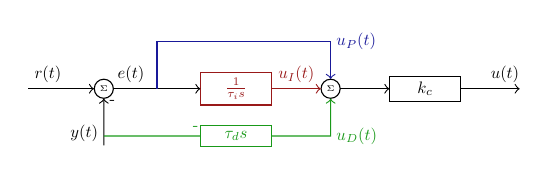
\begin{tikzpicture}[node distance=22mm, block/.style={rectangle, draw, minimum width=15mm}, sumnode/.style={circle, draw, inner sep=2pt}, scale=0.6, every node/.style={scale=0.6}]

    \node[coordinate] (input) {};
    \node[sumnode, right of=input, node distance=16mm] (sum) {\tiny $\Sigma$};
    \node[color=iic,block, right of=sum, node distance=28mm] (ii)  {$\frac{1}{\tau_is}$};
    \node[color=ppc, coordinate, above of=ii, node distance=10mm] (pp)  {};
    \node[color=ddc,block, below of=ii, node distance=10mm] (dd)  {$\tau_ds$};
    \node[sumnode, right of=ii, node distance=20mm] (sum2) {\tiny $\Sigma$};
    \node[block, right of=sum2, node distance=20mm] (gain)  {$k_c$};
    \node[coordinate, below of=sum, node distance=12mm] (feedback) {};
    \node[coordinate, right of=gain, node distance=20mm] (output) {};

    \draw[->] (input) -- node[above, pos=0.3] {$r(t)$} (sum);
    \draw[->] (sum) -- node[above, pos=0.2] {$e(t)$} node[coordinate] (mm) {}  (ii);
    \draw[->] (gain) -- node[above, near end] {$u(t)$} (output);
    \draw[->] (feedback) -- node[left, near start] {$y(t)$} node[right, pos=0.95] {-} (sum);
    \draw[->, color=ppc] (mm) |- (pp) -| node[right,] {$u_P(t)$} (sum2);
    \draw[->, color=ddc] (feedback |- dd) -- node[above, pos=0.95] {-} (dd) -| node[right,] {$u_D(t)$}   (sum2);
    \draw[->, color=iic] (ii)  -- node[above,] {$u_I(t)$} (sum2);
    \draw[->] (sum2) -- node[above, near end] {} (gain);

  \end{tikzpicture}
  \small
  \(  u(t) = k_c\Big( \textcolor{ppc}{e(t)} + \textcolor{iic}{\overbrace{\frac{1}{\tau_i} \int_0^{t} e(\xi) d\xi}^{u_I(t)}} + \textcolor{ddc}{ \underbrace{\tau_d \frac{d}{dt} \big(-y(t)\big)}_{u_D(t)}} \Big)\)
\end{center}

   \begin{center}
   \def\wn{2}
   \def\zz{0.3}
   \pgfmathsetmacro{\wwd}{\wn*sqrt(1-\zz*\zz)}
   \pgfmathsetmacro{\zwn}{\zz*\wn}
  \pgfmathsetmacro{\thangle}{acos(\zz)}
   \begin{tikzpicture}
   \begin{axis}[
    clip=false,
    width=14cm,
    height=4.5cm,
    ylabel={},
    xlabel={$t$},
    ymax = 2,
    ymin = -0.5,
    ]
      \addplot[black, no marks, domain=-0.4:8, samples=200] {(x>0)*(1 - exp(-x * \zwn)/sqrt(1-\zz*\zz) * sin(deg(\wwd*x) + \thangle))} node[coordinate, pin=20:{$y(t)$}, pos=0.3] {};
      \addplot[magenta!70!black, no marks, domain=-0.4:8, samples=200] coordinates {(-0.4, 0) (0,0) (0,1) (8,1)} node[coordinate, pin=90:{$r(t)$}, pos=0.2] {};
    \end{axis}

 \end{tikzpicture}
\end{center}

\alert{Activity} Sketch the error signal \(e(t)\) and the integral signal \(u_I(t)\) (use \(\tau_i=1\))
\end{frame}

\begin{frame}[label={sec:org642bfac}]{The PID - Integral signal - Solution}
   \def\wn{2}
   \def\zz{0.3}
   \pgfmathsetmacro{\wwd}{\wn*sqrt(1-\zz*\zz)}
   \pgfmathsetmacro{\zwn}{\zz*\wn}
  \pgfmathsetmacro{\thangle}{acos(\zz)}
\pgfplotstablenew[ create on use/x/.style={ create col/expr={\pgfplotstablerow/50} },    create on use/y/.style={ create col/expr={ exp(-\thisrow{x} * \zwn)/sqrt(1-\zz*\zz) * sin(deg(\wwd*\thisrow{x}) + \thangle)} }, create on use/int/.style={       create col/expr={\pgfmathaccuma+(\thisrow{y}+\prevrow{y})/2*(\thisrow{x}-\prevrow{x})} }, columns={x,y,int}]{400} \pidtable



\begin{center}
  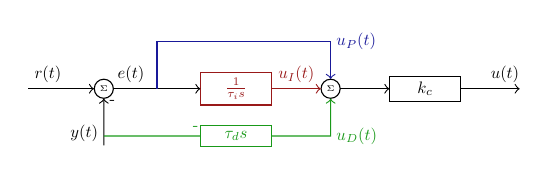
\begin{tikzpicture}[node distance=22mm, block/.style={rectangle, draw, minimum width=15mm}, sumnode/.style={circle, draw, inner sep=2pt}, scale=0.6, every node/.style={scale=0.6}]

    \node[coordinate] (input) {};
    \node[sumnode, right of=input, node distance=16mm] (sum) {\tiny $\Sigma$};
    \node[color=iic,block, right of=sum, node distance=28mm] (ii)  {$\frac{1}{\tau_is}$};
    \node[color=ppc, coordinate, above of=ii, node distance=10mm] (pp)  {};
    \node[color=ddc,block, below of=ii, node distance=10mm] (dd)  {$\tau_ds$};
    \node[sumnode, right of=ii, node distance=20mm] (sum2) {\tiny $\Sigma$};
    \node[block, right of=sum2, node distance=20mm] (gain)  {$k_c$};
    \node[coordinate, below of=sum, node distance=12mm] (feedback) {};
    \node[coordinate, right of=gain, node distance=20mm] (output) {};

    \draw[->] (input) -- node[above, pos=0.3] {$r(t)$} (sum);
    \draw[->] (sum) -- node[above, pos=0.2] {$e(t)$} node[coordinate] (mm) {}  (ii);
    \draw[->] (gain) -- node[above, near end] {$u(t)$} (output);
    \draw[->] (feedback) -- node[left, near start] {$y(t)$} node[right, pos=0.95] {-} (sum);
    \draw[->, color=ppc] (mm) |- (pp) -| node[right,] {$u_P(t)$} (sum2);
    \draw[->, color=ddc] (feedback |- dd) -- node[above, pos=0.95] {-} (dd) -| node[right,] {$u_D(t)$}   (sum2);
    \draw[->, color=iic] (ii)  -- node[above,] {$u_I(t)$} (sum2);
    \draw[->] (sum2) -- node[above, near end] {} (gain);

  \end{tikzpicture}
  \small
  \(  u(t) = k_c\Big( \textcolor{ppc}{e(t)} + \textcolor{iic}{\overbrace{\frac{1}{\tau_i} \int_0^{t} e(\xi) d\xi}^{u_I(t)}} + \textcolor{ddc}{ \underbrace{\tau_d \frac{d}{dt} \big(-y(t)\big)}_{u_D(t)}} \Big)\)
\end{center}

   \begin{center}
   \def\wn{2}
   \def\zz{0.3}
   \pgfmathsetmacro{\wwd}{\wn*sqrt(1-\zz*\zz)}
   \pgfmathsetmacro{\zwn}{\zz*\wn}
  \pgfmathsetmacro{\thangle}{acos(\zz)}
   \begin{tikzpicture}
   \begin{axis}[
    clip=false,
    width=14cm,
    height=4.5cm,
    ylabel={},
    xlabel={$t$},
    ymax = 2,
    ymin = -0.5,
    ]
      \addplot[black, no marks, domain=-0.4:8, samples=200] {(x>0)*(1 - exp(-x * \zwn)/sqrt(1-\zz*\zz) * sin(deg(\wwd*x) + \thangle))} node[coordinate, pin=20:{$y(t)$}, pos=0.3] {};
      \addplot[color=ppc, no marks, domain=-0.4:8, samples=600] {(x>0)*(exp(-x * \zwn)/sqrt(1-\zz*\zz) * sin(deg(\wwd*x) + \thangle))} node[coordinate, pin=200:{$e(t)$}, pos=0.3] {};
      \addplot [color=iic, thick] table [y=int] {\pidtable};
      \addplot[magenta!70!black, no marks, domain=-0.4:8, samples=200] coordinates {(-0.4, 0) (0,0) (0,1) (8,1)} node[coordinate, pin=90:{$r(t)$}, pos=0.2] {};
    \end{axis}

 \end{tikzpicture}
\end{center}
\end{frame}

\section{Windup}
\label{sec:orgdc284b6}

\begin{frame}[label={sec:org744d11d}]{Integral windup}
\href{https://tecdemonterrey.instructuremedia.com/embed/6fb197b1-38a6-4938-b622-b25d4a45efcc}{Video by Tomás Alejandro Lugo Salinas (MTY)} 
\end{frame}

\section{Anti-windup}
\label{sec:org744d659}

\begin{frame}[label={sec:org60c71b8}]{Anti-windup using back-calculation}
\begin{center}
\includegraphics[width=1.02\linewidth]{../../figures/anti-windup-back-calculation.png}
\end{center}
\end{frame}
\end{document}